\documentclass{beamer}
\usepackage[spanish]{babel}
\usepackage[utf8]{inputenc}
\usepackage{graphicx}

\newtheorem{definicion}{Definición}
\newtheorem{ejemplo}{Ejemplo}

\usetheme{classic}


\title[Título]{Interpolación de Taylor}
\author[Autores]{Mérari Afonso\\
				 Ignacio Fragoso\\
                 Lidia García}
\date{\today}


\begin{document}
  
%++++++++++++++++++++++++++++++++++++++++++++++++++++++++++++++++++++++++++++++
\begin{frame} %Para poner imágenes
\maketitle
 % \includegraphics[width=0.15\textwidth]{img/ullesc.eps}
 % \hspace*{7.5cm}
 % \includegraphics[width=0.16\textwidth]{img/fmatesc.eps}
 % \titlepage

  \begin{scriptsize}
    \begin{center}
     
    \end{center}
  \end{scriptsize}

\end{frame}

%+++++++++++++++++++++++++++++++++++++++++++++++++++++++++++++++++++++++++++++ 
\begin{frame}
  \frametitle{Índice}  
  \tableofcontents[pausesections]
\end{frame}
%++++++++++++++++++++++++++++++++++++++++++++++++++++++++++++++++++++++++++++++

\section{Introducción} 
\begin{frame}
  \frametitle{Información del sistema operativo y del compilador}
	\begin{itemize}
	   \item La versión de Python utilizada es:\\	
		Python 2.7.3 \\ 
       \pause
	   \item Información del sistema operativo: \\
		'Linux', 'ubuntu', '3.5.0-17-generic'
	   \pause
       \item Información del procesador del sistema:\\
		model name: Intel(R) Celeron(R) CPU  550  @ 2.00GHz\\
		cpu MHz: 1995.123\\
		cache size: 1024 KB\\
	\end{itemize}
\end{frame}

%+++++++++++++++++

\section{Interpolación de Taylor}
\begin{frame}
	\frametitle{Procedimiento}
		\centerline {Nuestra función es: {\LARGE $cos(\pi x)$ }en [1,2]}\
        \begin{itemize}
        \item Para hallar la interpolación de Taylor hemos utilizado el polinomio de Taylor
        \[P(x)=\sum\limits_{i=1}^n\frac{f^{(i)}(x_0)}{i!}\quad(x-x_0)^i \]
        \pause
		\item Para hallar el error restamos el valor real de la función menos el valor de la interpolación de Taylor en valor absoluto.
		\end{itemize}
\end{frame}
%+++++++++++++++++++++++++++++++++++++++++++++++++++++++++++++++++++
\begin{frame}
  \frametitle{Resultados Obtenidos}
	Fijando el valor de x y la derivada n-ésima (x=1, n=5)\\
	\begin{center}
	\begin{tabular}{||c|c|c|c||}
	\hline
    \hline
	Centro & Interpolación Taylor & Valor Real & Error \\
	\hline
	1.0 & -1 & -1 & 0\\
	\hline
	1.25 & -1.00025363221339 & -1 & 0.000253632213394583 \\
	\hline
	1.5 & -1.00452485553482 & -1 & 0.00452485553481630\\	
	\hline
	1.75 & -0.900045035338955 & -1 & 0.0999549646610447\\
	\hline
	2 & 0.123909925872083 & -1 & 1.12390992587208\\
	\hline
    \hline
	\end{tabular}
    \end{center}
\end{frame}

\begin{frame}
	Fijando el centro y la n-ésima (c=1.5, n=1)\
    \begin{center}
	\begin{tabular}{||c|c|c|c||}
	\hline
    \hline
	x & Int. Taylor & Valor Real & Error \\
	\hline
	-1.5 & -352.175700107991 & -1.8369701e-16 & 352.1757 \\
	\hline
	0.0 & -3.40445153931272 & 1 & 4.4044515393127 \\
	\hline
	1.0 & -1.00025363221339 & -1 & 0.00025363221339458\\	
	\hline
    1.5 & -0.000202346334410 & -1.8369701e-16 & 0.00020234633441002\\
    \hline
    3 & -3.03724338394450 & -1 & 2.0372433839445\\
    \hline
    \hline
	\end{tabular}
    \end{center}
\end{frame}
\begin{frame}
	Fijando el valor del centro y el valor de x (c= 1.5, x=1)
	\begin{center}
	\begin{tabular}{||c|c|c|c||}
	\hline
    \hline
	n-ésima & Interpolación Taylor & Valor Real & Error \\
    \hline
	3 & -0.924832229288648 & -1 & 0.075167770711351\\
	\hline
    8 & -0.999843101399498 & -1 & 0.000156898600502386\\
    \hline
    10 & -1.00000354258429 & -1 & 3.54258428503229e-6 \\
    \hline
    17 & -1.00000000000004 & -1 & 4.26325641456060e-14\\
	\hline
	20 & -0.999999999999999 & -1 & 1.1102302462516e-15\\	
	\hline
    \hline
	\end{tabular}
	\end{center}
\end{frame}
%++++++++++++++++++++++++++++++++++++++++++++++++++++++++++++++
\begin{frame}
 Gráfica calculada para la n-ésima 2
 \begin{center}
 \begin{figure}
   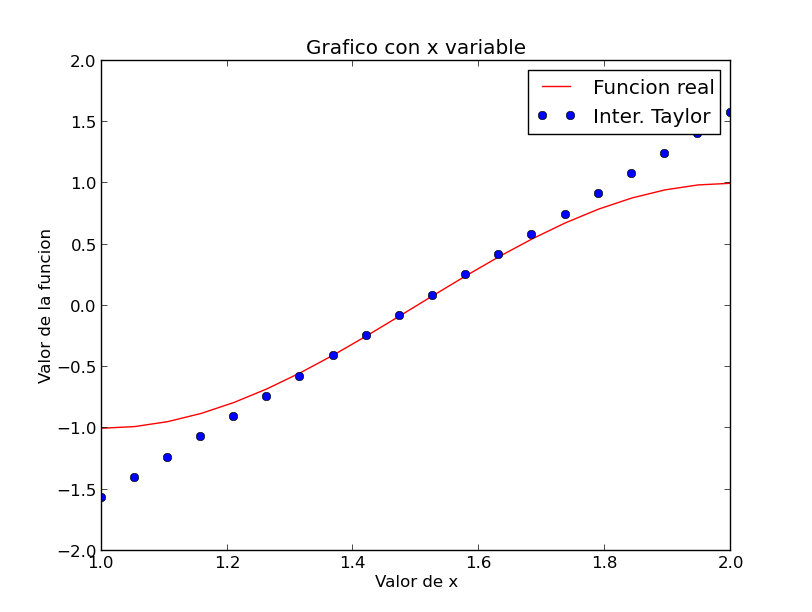
\includegraphics[scale=0.5]{grafica1.png}
   %\hspace*{7.5cm}
 \end{figure}
 \end{center}
\end{frame}
%++++++++++++++++++++++++++++++++++++++++++++++++++++++++
\begin{frame}
 Gráfica calculada para la n-ésima 20
 \begin{center}
 \begin{figure}
   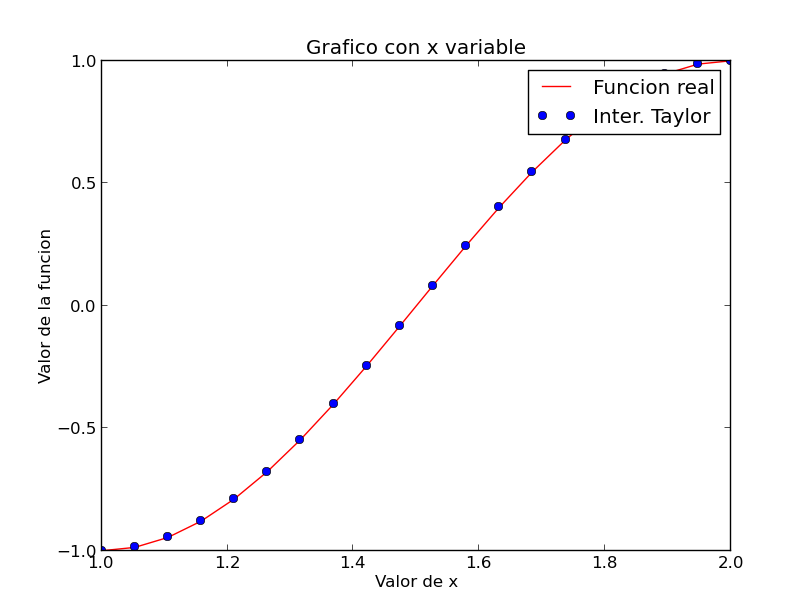
\includegraphics[scale=0.5]{grafica2.png}
 \end{figure}
 \end{center}
\end{frame}
%++++++++++++++++++++++++++++++++++++++++++++++++++++++++++
\begin{frame}

	\centerline{\Huge FIN}
\end{frame}
\end{document}

